% Created 2024-09-08 Sun 07:26
% Intended LaTeX compiler: pdflatex
\documentclass[letterpaper, 12pt]{article}
                                \usepackage{lmodern} % Ensures we have the right font
\usepackage[T1]{fontenc}
\usepackage[utf8]{inputenc}
\usepackage{graphicx}
\usepackage{amsmath, amsthm, amssymb}
\usepackage[table, xcdraw]{xcolor}
\usepackage{tikz}
\usetikzlibrary{automata, positioning, arrows}
\renewcommand{\thesection}{\Roman{section}}
\renewcommand{\thesubsection}{}
\renewcommand{\thesubsubsection}{}
\definecolor{bblue}{HTML}{0645AD}
\usepackage[colorlinks]{hyperref}
\hypersetup{colorlinks, linkcolor=blue, urlcolor=bblue}
\usepackage{titling}
\setlength{\droptitle}{-6em}
\setlength{\parindent}{12pt}
\setlength{\parskip}{0em}
\usepackage[stretch=10]{microtype}
\usepackage{hyphenat}
\usepackage{ragged2e}
\usepackage{subfig} % Subfigures (not needed in Org I think)
\usepackage{hyperref} % Links
\usepackage{listings} % Code highlighting
\usepackage[top=1in, bottom=1.00in, left=0.85in, right=0.85in]{geometry}
\renewcommand{\baselinestretch}{1.00}
\usepackage[explicit]{titlesec}
\pretitle{\begin{center}\fontsize{20pt}{20pt}\selectfont}
\posttitle{\par\end{center}}
\preauthor{\begin{center}\vspace{-6bp}\fontsize{12pt}{12pt}\selectfont}
\postauthor{\par\end{center}\vspace{-25bp}}
\predate{\begin{center}\fontsize{12pt}{12pt}\selectfont\vspace{1em}}
\postdate{\par\end{center}\vspace{0em}}
\titlespacing\section{0pt}{5pt}{5pt} % left margin, space before section header, space after section header
\titlespacing\subsection{0pt}{5pt}{2pt} % left margin, space before subsection header, space after subsection header
\titlespacing\subsubsection{0pt}{5pt}{-2pt} % left margin, space before subsection header, space after subsection header
\usepackage{enumitem}
\setlist{itemsep=-2pt} % or \setlist{noitemsep} to leave space around whole list
\usepackage{listings}
\author{Jackson Mowry}
\date{\textit{<2024-09-08 Sun>}}
\title{Hw1}
\hypersetup{
 pdfauthor={Jackson Mowry},
 pdftitle={Hw1},
 pdfkeywords={},
 pdfsubject={},
 pdfcreator={Emacs 29.4 (Org mode 9.8)}, 
 pdflang={English}}
\begin{document}

\maketitle
\tableofcontents

\section{Problem 1}
\label{sec:org04bcb37}
\begin{enumerate}
\item \{w | w has at least 2 a's and at least 3 b's\}
\end{enumerate}
\begin{center}
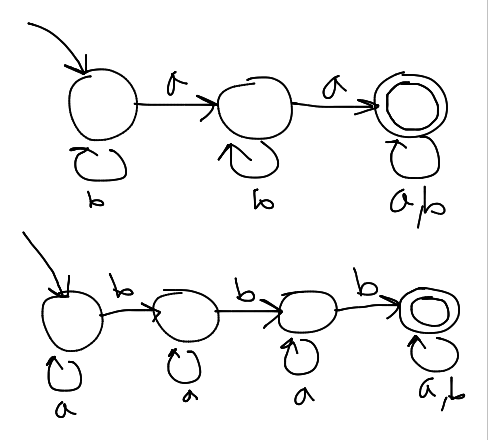
\includegraphics[width=6cm]{hw2/simple1-1.png}
\end{center}
\begin{center}
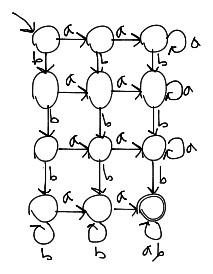
\includegraphics[width=6cm]{hw2/1-1.png}
\end{center}
simple, then final

\begin{enumerate}
\item \{w | w has an odd number of a's and no more than 2 b's\}
\end{enumerate}
\begin{center}
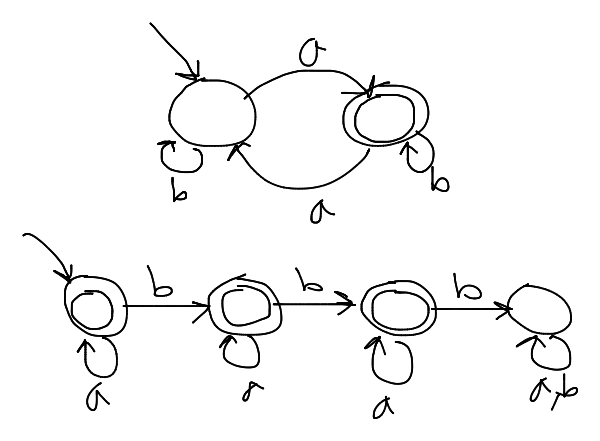
\includegraphics[width=6cm]{hw2/simple1-2.png}
\end{center}
\begin{center}
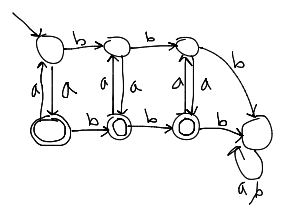
\includegraphics[width=6cm]{hw2/1-2.png}
\end{center}
simple, then final

\begin{enumerate}
\item \{w | w starts with the character b and has at most 1 a\}
\end{enumerate}
\begin{center}
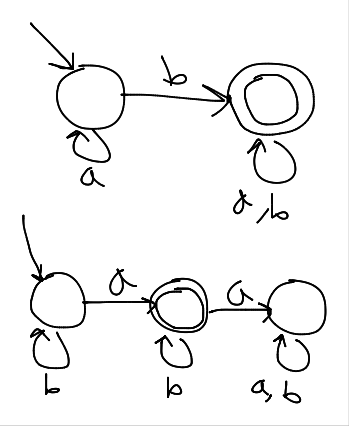
\includegraphics[width=6cm]{hw2/simple1-3.png}
\end{center}
\begin{center}
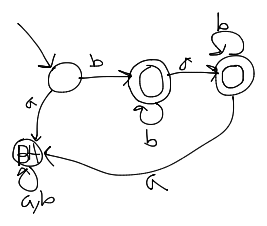
\includegraphics[width=6cm]{hw2/1-3.png}
\end{center}
simple, then final
\section{Problem 2}
\label{sec:orgfb43a52}
\begin{enumerate}
\item \{w | w contains neither the substring aa nor the substring bb\}
\end{enumerate}
\begin{center}
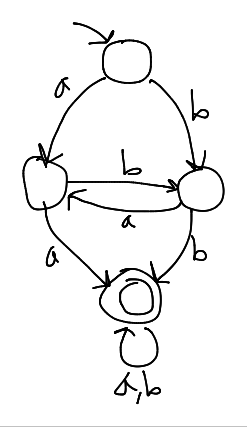
\includegraphics[width=4.5cm]{hw2/simple2-1.png}
\end{center}
\begin{center}
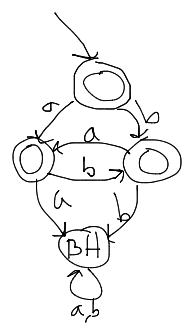
\includegraphics[width=4.5cm]{hw2/2-1.png}
\end{center}
Simple first, final last

\begin{enumerate}
\item \{w | w is any string not in b\textsuperscript{*}a\textsuperscript{*}\}
\end{enumerate}
\begin{center}
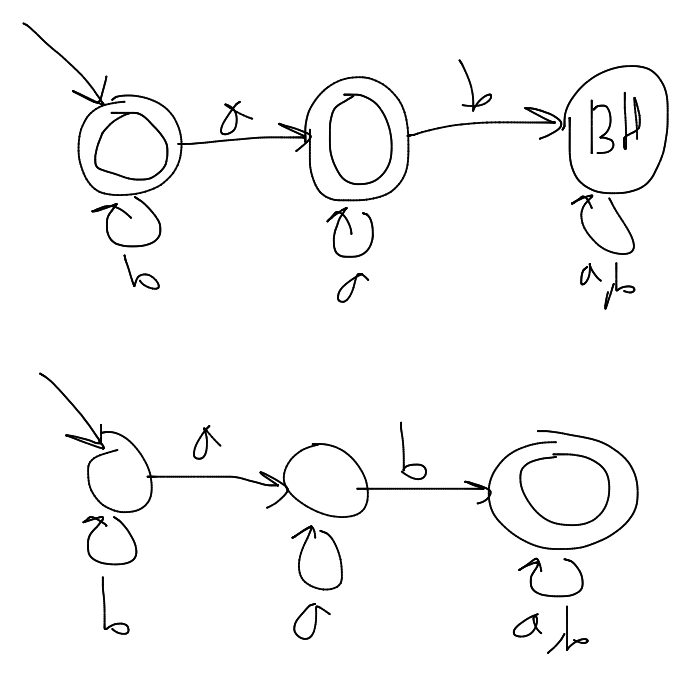
\includegraphics[width=8cm]{hw2/2-2.png}
\end{center}
Simple top, final bottom

\begin{enumerate}
\item \{w | w is any string not in (ab\textsuperscript{+}a)\textsuperscript{*}\}
\end{enumerate}
\begin{center}
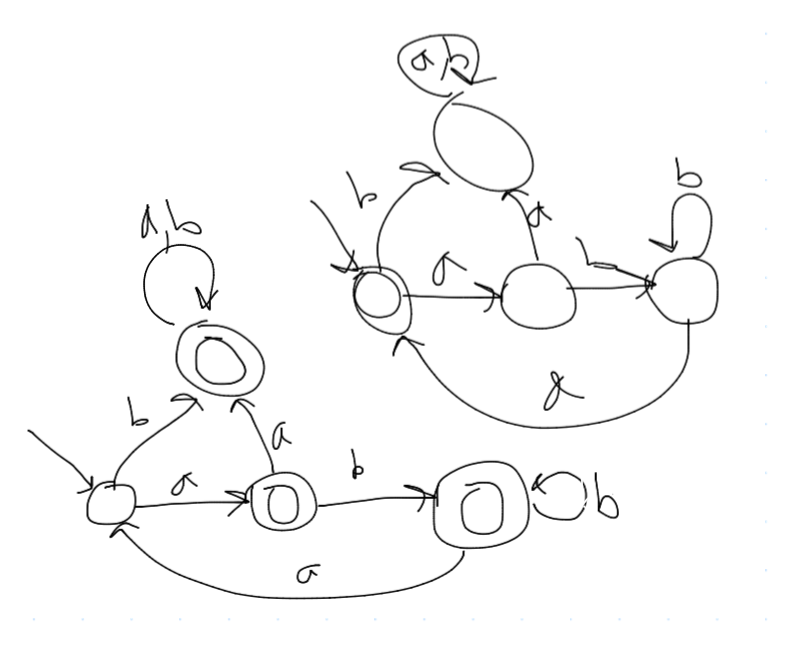
\includegraphics[width=8cm]{hw2/2-3.png}
\end{center}
Simple top right, final bottom left
\end{document}
